\section{Un ejemplo de Alexander}

\comm{Davenma y Venema}

\comm{En la claim 2.1.5 usar la descomposición de heegaard de $\R^3$ como dos toros}

\comm{Al final de los ejemplos hablar de que tomar suspensión me da ejemplos de dim superior. Esto está en DV después de Alexander.}

En esta sección vamos a dar un ejemplo de una bola encajada en $\R^3$ tal que el encaje no se extiende a un homeomorfismo de todo $\R^3$. 

Podemos construir la imagen como una intersección numerable de cerrados encajados $\{X_n\}$. Para el resto de la construcción, va a ser conveniente definir los siguientes conjuntos auxiliares: 

Sea $T$ un toro sólido en $\R^3$ dado por un encaje $\varphi :\s^1\times \D^2\rightarrow \R^3$ y sea $[t_1,t_2]\subset \s^1$ un intervalo cerrado. Llamamos $\textbf{cilindro contenido en T}$ al conjunto $C:=\varphi([t_1,t_2]\times \D^2)$, y decimos que los dos discos $\varphi(\{t_1\}\times\D^2)$, $\varphi(\{t_2\}\times\D^2)$ son las \textbf{tapas del cilindro}.

Dado un cilindro $C$, lo que nos va a interesar en general es considerar dos toros sólidos $T'$ y $T''$ que estén contenidos en $C$, enlazados entre ellos (con un enlace simple) y con $T'\cap \partial C=\tau_1$, $T''\cap \partial C=\tau_2$ como en la imagen $\ref{alex1}$. Llamaremos $\textbf{toros enlazados en C}$ a dos toros que cumplen lo anterior.

\comm{los toros tienen número de enlace 1, ver si defino número de enlace o cómo digo eso. todos los enlaces que voy a usar siempre van a ser simples, o sea van a tener número de enlace 1. seguro esta construcción se puede hacer con número de enlace arbitrario y tiene pinta que quedan no equivalentes}

\begin{figure}[h!]
    \centering
    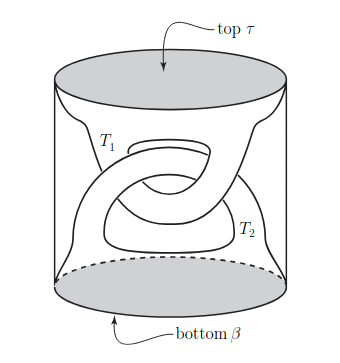
\includegraphics[width=0.5\linewidth]{img mono/alexander/1.png}
    \caption{Un cilindro conteniendo $T_1$ y $T_2$}
    \label{alex1}
\end{figure}

Ahora si, vamos a definir nuestra sucesión de cerrados encajados: 

Empezamos por $X_0$ un toro sólido estándar en $\R^3$, con diámetro menor a $1$. Consideramos un cilindro $C$ contenido en $X_0$ con diámetro menor a $\frac{1}{2}$, y llamamos $T_0$ y $T_1$ a dos toros enlazados en $C$. Definimos \begin{align*}
    B_0&:=X_0 - C \\
    X_1&:=B_0\cup T_0\cup T_1
\end{align*} Observar que $B_0$ es el toro sólido estándar sin un cilindro $C$, por lo tanto $B_0$ es homeomorfo a un disco $\D^3$.

Para definir $X_2$, vamos a modificar sólamente los toros $T_0$ y $T_1$, y lo haremos de la misma forma en la que modificamos el toro $X_0$ en el paso anterior. Lo que hacemos es considerar $C_0\subset T_0$ y $C_1\subset T_1$ dos cilindros contenidos en $T_0$ y $T_1$ respectivamente. Esta vez procuramos que estos cilindros no intersecten a las tapas del cilindro anterior $C$, y que además tengan diámetros menores a $\frac{1}{4}$. Consideramos $T_{00}, T_{01}\subset C_0$ y $T_{10}, T_{11}\subset C_1$ toros enlazados en $C_0$ y $C_1$ respectivamente. Definimos \begin{align*} B_1&:= X_1-(C_0\cup C_1)\\
    X_2&:=B_1\cup\bigg(\bigcup\limits_{i,j\in\{0,1\}} T_{ij}\bigg)\end{align*}

El resto de la sucesión lo definimos inductivamente. Asumamos que en el paso $n$ se eliminaron los $2^{n-1}$ cilindros $\{C_\alpha : \alpha\in \{0,1\}^{n-1}\}$ de diámetro menor a $2^{-(n-1)}$ y se reemplazaron por los $2^n$ toros sólidos $\{T_\beta : \beta\in \{0,1\}^{n}\}$. 

Lo primero que hacemos para definir $X_{n+1}$ es considerar un cilindro $C_\beta$ contenido en cada $T_\beta$. Procuramos que este $C_\beta$ tenga diámetro menor a $2^{-n}$ y que no intersecte las tapas del cilindro $C_\alpha$ en el que $T_\beta$ estaba contenido.

Ahora para cada $\beta\in\{0,1\}^n$ consideramos $T_{\beta 0}$ y $T_{\beta 1}$ dos toros enlazados en $C_\beta$. Identificamos $\beta 0$ y $\beta 1$ con los elementos de $\{0,1\}^{n+1}$ que coinciden con $\beta$ en los primeros $n$ lugares y son $0$ o $1$ en el último, respectivamente.

Definimos entonces $X_{n+1}$ como $$X_{n+1}:=\bigg[X_n-\bigg(\bigcup\limits_{\beta\in\{0,1\}^n} C_\beta \bigg)\bigg]\cup\bigg( \bigcup\limits_{\gamma\in\{0,1\}^{n+1}}T_\gamma\bigg)$$

Llamamos a $B=\bigcap\limits_{n=1}^\infty X_n$ la \textbf{bola de Alexander}.

\duda{acá hay un detalle que no dije que es que los subtoros enlazados hay que tomarlos con cuidado para que después pueda considerar un cilindro contenido en cada uno con el diámetro acotado como quiero. si tomara los subtoros super gordos no me sirve aa}

Todavía no probamos que efectivamente este espacio es una bola. Antes de hacer eso, vamos a definir el mismo conjunto como una unión encajada en vez de una intersección.

% Llamamos $S=\partial B$ la esfera de Alexander. 

Veamos que $\pi_1(B^c)$ es no trivial: Recordamos la definición de $B$ como unión de conjuntos $X_n$.Tomamos $J$ una curva cerrada que sea no trivial en el complemento del toro $X_0$. Supongamos $J$ es trivial en $B^c$ y consideramos su homotopía $H$ a un punto. 
            
El conjunto $\im(H)$ es un compacto contenido en $B^c$. Observar que $B^c$ cumple $$B^c=\left(\bigcap\limits_{n=1}^\infty X_n\right)^c=\bigcup\limits_{n=1}^\infty X_n^c$$ 
Como $\{X_n^c\}$ cubre $\im(H)$, entonces existe un subcubrimiento finito $\{X_1^c,\dots, X_N^c\}$ para algún $N\in\N$. Observar que todos los $\{X_n\}$ son cerrados y cumplen $X_{n+1}\subset X_n$. Por lo tanto, la familia $\{X_n^c\}$ está compuesta por abiertos encajados. Por esta razón podemos reducir el subcubrimiento $\{X_1^c,\dots, X_N^c\}$ a uno compuesto únicamente por el elemento $X_N^c$. 

Encontramos entonces un $N\in\N$ tal que $\im(H)\subset X_N^c$, es decir, $J$ es contractible en $X_N^c$. Por inducción podemos ver que esto es absurdo. \comm{falta agregar esto}

Ahora veamos que $B$ es una bola: Pensemos $B$ como unión de cosas en vez de intersección, y veamos que estas consturcciones nos dan el mismo conjunto. 

Definimos inductivamente una familia $\{B_n\colon n\in\N\}$ de conjuntos encajados $B_{n}\subset B_{n+1}$. Empezamos por definir $$B_0:= X_0 - C$$ este conjunto es el toro sólido estándar $X_0$ sin el cilindro $C$, por lo tanto $B_0$ es homeomorfo a un disco $\D^3$.

Para definir $B_1$, consideramos $X_1$

Ahora, asumiendo que tenemos $B_n$, definamos $B_{n+1}$.

En el pasaje de la etapa $n$ a la etapa $n+1$ de la construcción, ubicamos en el conjunto $X_n$ un total de $2^{n}$ cilindros $C_\alpha$. Definimos el siguiente conjunto, al que llamamos \textbf{bola con n cuernos}: $$B_n :=X_n - \bigcup\limits_{\alpha\in\{0,1\}^{n}}C_\alpha$$ 

Tenemos entonces $2^n$ toros sólidos en la etapa $n$, que son cada uno unión de una pillbox y una 3-célula complementaria. 

Si llamamos $D_n$ a la unión de las $2^{n-1}$ 3-células complementarias a las $2^{n-1}$ pillboxes en la etapa $n$ de la construcción. 

De esta manera podemos definir $B$ como $\overline{\bigcup\limits_{n=1}^\infty C_n}$, siendo $C_1=D_1$ y $C_n=C_{n-1}\cup D_n$ 
            
\duda{convencerme de por qué preciso clausurar--> $B$ es intersección arbitraria de cerrados entonces es cerrado, los $C_n$ son abiertos entonces su unión va a ser abierta. Como $B$ no es $\varnothing$ ni $\R^3$ no puede ser un clopen, entonces no son iguales. Falta convencerme pq clausurar funciona.} 

Llamemos $P_n^i$ a la i-ésima pillbox del n-ésimo paso de la construcción. Es decir, $P_n^i\subset X_n \fall i\in\{1,\dots,2^{n-1}\}$ y $X_n=X_{n+1}\cup\bigcup\limits_{i=1}^{2^{n-1}}P_n^i$. 
            
Sea $x\in B-\bigcup\limits_{n=1}^\infty C_n \Rightarrow x\in \bigcap\limits_{n=1}^\infty X_n-\bigcup\limits_{n=1}^\infty C_n$ 

$x\not\in\bigcup\limits_{n=1}^\infty C_n \Rightarrow x\not\in C_n\fall n\in\N$ 

$x\in B-C_n\Rightarrow \exst i\in\{1,\dots,2^{n-1}\}$ tal que $x\in P_n^i$ 

Con esto concluimos que $x\in B-\bigcup\limits_{n=1}^\infty C_n \Leftrightarrow x\in\bigcap\limits_{n=1}^\infty P_n^{k_n}$ para alguna sucesión de naturales $\{k_n\}$. \comm{recordar que $diam(P_n)\xrightarrow{n} 0$, son compactas y encajadas}

Como $diam(P_n)\xrightarrow{n} 0$, esto además implica que $x\in\overline{\bigcup\limits_{n=1}^\infty C_n}$, y por lo tanto tenemos la igualdad de conjuntos. 

Además, fun fact, observar que dada una pillbox $P_n^i$ se cumple que $\#\big\{j\in\{1,\dots, 2^n\}:P_{n+1}^j\cap P_n^i\neq\varnothing\big\}=2$, por lo tanto, los $x\in B-\bigcup\limits_{n=1}^\infty C_n$ están en biyección con $2^{\N}$, es decir, son un Cantor. 

Viendo $B$ de esta manera, probemos que efectivamente es una bola: 

Para cada $C_n$ en la construcción, podemos definir un homeo $h_n:C_n\to C_{n+1}$ soportado en un entorno $U_n$ de $C_n\cap D_{n+1}$. 

Definimos entonces una familia de funciones $\{f_n:C_1\to C_{n+1}\}_{n\in\N}$ tales que $f_n=h_n\circ h_{n-1}\circ\dots\circ h_1$. Observar que cada $f_n$ difiere de $f_{n+1}$ sólamente en $U_n$.

Como $diam(P_n)\xrightarrow n 0$, podemos ir tomando los $U_n$ con $diam(U_n)\xrightarrow n 0$, por lo tanto $\{f_n\}$ converge uniformemente a $f:C_1\to B$, que resulta continua. \comm{acomodar esto pq en realidad los $U_n$ son disconexos entonces el diametro no tiende a 0}

Queremos verificar ahora que $f$ es biyectiva, y con eso obtener que es un homeomorfismo. 

Por lo visto anteriormente, sabemos que $K=f^{-1}(B-\bigcup\limits_{n=1}^{\infty}C_n)$ es un conjunto de Cantor. 

Dado $x\in C_1- K$, $\exst N\in\N$ tal que $f_{N-1}(x)\in C_{N}-U_N$ (en este caso pensamos $f_0$ como la identidad), y por lo tanto $f(x)=f|_{N-1}(x)$. 
            
Con esto tenemos que $f$ es biyectiva en $C_1- K$. 

Por lo observado anteriormente, dados $x_0, x_1\in K$, en algún momento van a estar en distintas componentes conexas de los entornos $U_n$, y por lo tanto van a diferir sus imágenes por alguna de las $f_n$. Con esto tenemos la inyectividad de $f$ en $K$. 

Para la sobreyectividad, tomamos un punto $x\in B-\bigcup\limits_{n=1}^{\infty}C_n$ y su correspondiente elemento de $2^\N$, y observamos que se corresponde a un único punto \comm{terminar de escribir}
